\subsection{Minimax}
Minimax is a backtracking algorithm that is used to find the optimal move for a player in a zero-sum game. The two players are called maximizer and minimizer. The goal of the maximizer is to get the highest score possible while the goal of the minimizer is to do the opposite and get the lowest score possible. The first step of minimax algorithm is to build a game tree to search.\\
\\
For a gomoku game tree, each node represents a board state that has a value associated with it. This value is the score of that specific board state, calculated by a scoring function with the heuristics based on stone shapes. Stone shape considers two parts, the number of consecutive stones and the number of open ends. If there are two open ends, it is called live; otherwise, it is called dead. Therefore, there are 7 categories of stone shapes: five in a row, live four, dead four, live three, dead three, live two, dead two. Five in a row has the highest score, while dead two has the lowest score.\\
\\
The pseudo code of minimax is shown below. This is a recursive function, the base case is reached when the search depth has been reached or the game has ended.\\

\begin{algorithm}[!htbp]
\SetAlgoLined
\SetKwInOut{Input}{input}
\SetKwInOut{Output}{output}
\Input{node, depth, maximizingPlayer}
\Output{score}

\If{depth == 0 or node is a terminal node}{
    return the heuristic score of node\;
}
\eIf{maximizingPlayer}{
    value = -$\infty$\;
    \For{each child of node}{
        score = max(value, minimax(child, depth-1, false))\;
    }
    return score\;
}{
    score = $\infty$\;
    \For{each child of node}{
        score = max(value, minimax(child, depth-1, true))\;
    }
    return score\;
}
\caption{Minimax}
\label{alg:minimax}
\end{algorithm}


\subsection{Alpha-Beta Pruning}
Alpha-Beta is an optimization for minimax algorithm. It prunes the branches of the game tree that need not be searched because there already exists a better move. Alpha-Beta pruning gets its name from two bounds that are passed along during the calculation, which restrict the set of possible solutions based on the portion of the each tree that has already been seen.\\
\\
Alpha represents the maximum lower bound of possible solutions, and beta represents the minimum upper bound of possible solutions. To visualize, we can use a line to represent the possible solutions. Initially, alpha is set to be -$\infty$, and beta is set to be $\infty$. \\
\\
As the game tree is being searched, there will be more restrictions about the range of possible solutions based on the nodes it has already seen. The bounds will get closer and closer together.\\
\\
Finally, once alpha and beta no longer overlap \(\alpha\leq\beta\), we know that this node could never result in a solution path, so we may stop processing this node. Meaning, we will stop generating its children and move back to its parent node. This is shown in Figure~\ref{fig:alpha-beta}.\\

\begin{figure}[!htbp]
    \centering
    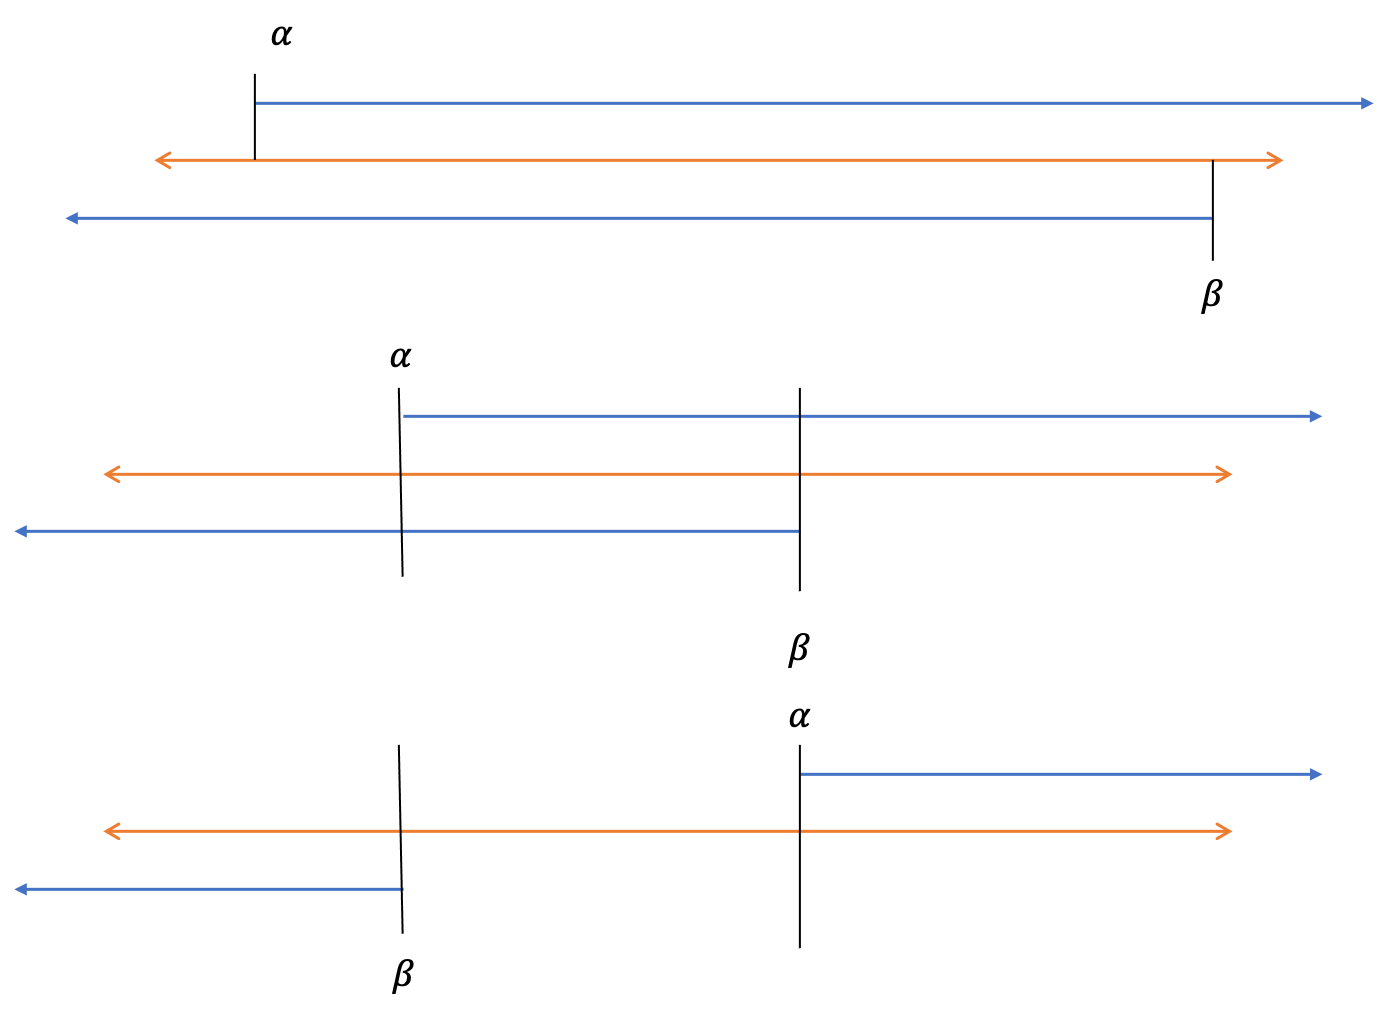
\includegraphics[scale=0.3]{images/ab.png}
    \caption{alpha and beta bounds}
    \label{fig:alpha-beta}
\end{figure}

\begin{algorithm}[!htbp]
\SetAlgoLined
\SetKwInOut{Input}{input}
\SetKwInOut{Output}{output}
\Input{node, depth, maximizingPlayer, alpha, beta}
\Output{score}

\If{depth == 0 or node is a terminal node}{
    return the heuristic score of node\;
}
\eIf{maximizingPlayer}{
    value = -$\infty$\;
    \For{each child of node}{
        score = max(value, minimax(child, depth-1, false, alpha, beta))\;
        alpha = max(alpha, score)\;
        \If{alpha $\leq$ beta}{
            break\;
        }{}
    }
    return score\;
}{
    score = $\infty$\;
    \For{each child of node}{
        score = max(value, minimax(child, depth-1, true, alpha, beta))\;
        beta = min(beta, score)\;
        \If{beta $\leq$ alpha}{
            break\;
        }{}
    }
    return score\;
}
\caption{Minimax with alpha-beta pruning}
\label{alg:minimaxab}
\end{algorithm}

\noindent
Algorithm~\ref{alg:minimaxab} is the pseudo code for the minimax algorithm with the inclusion of alpha-beta pruning. Note that the initial call to minimax with alpha-beta pruning sets alpha and beta to $-\infty$ and $+\infty$ respectively.


\subsection{Calculating the Best Move}
With the minimax algorithm and alpha-beta pruning defined, we can use this to find the best move as follows. For a given initial board state $s$, we first gather all the possible moves that the current player. For this work, we have defined all possible moves to be any unoccupied board location. Alternatively, we could only consider a subset by choosing positions that are adjacent, either above, below or diagonally, to an already occupied board location. Next, for each one of those moves we can call Algorithm~\ref{alg:minimax} and yield a score for each potential move. Finally, the move  with the highest score can be returned as the best move. In the case that there are multiple moves with the highest score, any of those would suffice as the 'best' move. 